\subsection{Visualizzazione mobile}
\begin{figure}[H]
  \centering
  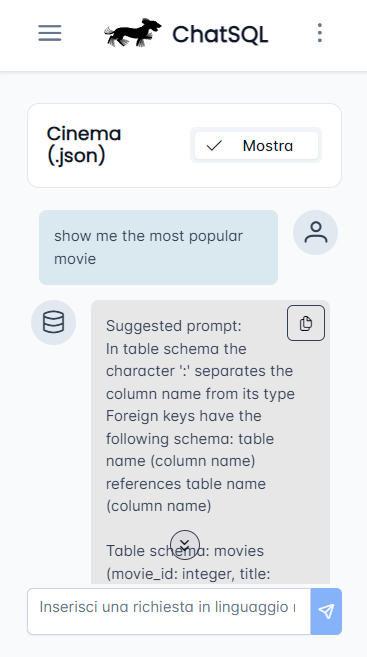
\includegraphics[width=0.50\textwidth]{assets/mobile.png}
  \caption{Versione mobile dell'applicazione}
\end{figure}
\par L'applicazione è stata progettata per essere fruibile anche da dispositivi mobili per garantire una buona esperienza d'uso con schermi touch screen di piccole dimensioni.  
\par Per migliorare la navigazione da dispositivi mobili, il menù principale, di default è nascosto e può essere aperto cliccando l'icona a tre linee 
\includegraphics[height=1.2em]{assets/dd_burger_menu.png} in alto a sinistra.
\par Le viste dell'applicazione occupano tutta la grandezza dello schermo, per dare più spazio possibile al contenuto principale.
\par Per ridurre l'ingombro dello schermo, i bottoni di login e delle impostazioni di sistema, sono accessibili mostrando un menù a tendina, cliccando sull'icona a tre puntini 
\includegraphics[height=1.2em]{assets/dd_kebab_menu.png} in alto a destra.